% Editable standalone vector figure extracted from novogaia_spectra.tex.
% Source slide 11; figure 11; native embedded fonts.
% Compile with LuaLaTeX from this directory, or run ../export_figures.py.
\documentclass[tikz,border=0pt]{standalone}
% Shared editable preamble for standalone, Nature-style vector figures.
% Text remains embedded and searchable. This is a house-style target, not a
% claim of acceptance or of satisfying every journal's submission checklist.
\usepackage{fontspec}
\setmainfont{LiberationSans}[
  Path=../assets/,Extension=.ttf,
  UprightFont=*-Regular,BoldFont=*-Bold,ItalicFont=*-Italic,BoldItalicFont=*-BoldItalic]
\setsansfont{LiberationSans}[
  Path=../assets/,Extension=.ttf,
  UprightFont=*-Regular,BoldFont=*-Bold,ItalicFont=*-Italic,BoldItalicFont=*-BoldItalic]
\setmonofont{LiberationSans}[
  Path=../assets/,Extension=.ttf,
  UprightFont=*-Regular,BoldFont=*-Bold,ItalicFont=*-Italic,BoldItalicFont=*-BoldItalic]
\usepackage{unicode-math}
\setmathfont{Latin Modern Math}
\DeclareMathSizes{5.9}{6}{5}{5}
\DeclareMathSizes{6}{6}{5}{5}
\usepackage{tikz}
\usetikzlibrary{arrows.meta,calc,positioning,patterns,decorations.pathreplacing,matrix}
\usepackage{graphicx}
\usepackage{xcolor}
\pagecolor{white}
\definecolor{ink}{HTML}{202020}
\definecolor{paper}{HTML}{FFFFFF}
\definecolor{muted}{HTML}{494949}
\definecolor{line}{HTML}{808080}
\definecolor{soft}{HTML}{F0F0F0}
\hyphenpenalty=10000\exhyphenpenalty=10000
\newcommand{\figurefont}{\sffamily\fontsize{5.9}{7.4}\selectfont}
\newcommand{\figuremathfont}{\sffamily\fontsize{6}{7.5}\selectfont}
\newcommand{\brandmedium}{\bfseries}
\renewcommand{\normalsize}{\figurefont}
\renewcommand{\small}{\figurefont}
\renewcommand{\footnotesize}{\figurefont}
\renewcommand{\scriptsize}{\figurefont}
\renewcommand{\tiny}{\figurefont}
\renewcommand{\large}{\figurefont}
\renewcommand{\Large}{\figurefont}
\renewcommand{\LARGE}{\figurefont}
\renewcommand{\huge}{\figurefont}
\renewcommand{\Huge}{\figurefont}
\tikzset{
  every path/.style={line width=.55pt},
  every node/.style={font=\figurefont,text=ink},
  arr/.style={-{Latex[length=1.5mm,width=1mm]},line width=.55pt,draw=ink},
  thinarr/.style={-{Latex[length=1.3mm,width=.9mm]},line width=.55pt,draw=ink},
  box/.style={draw=ink,line width=.55pt,fill=white,minimum height=.85cm,align=center,inner sep=3pt},
  ghost/.style={draw=muted,dashed,fill=soft},
  tag/.style={font=\figurefont,text=muted},
  equ/.style={font=\figuremathfont},
  small/.style={font=\figurefont},
  body/.style={font=\figurefont},
  tinytext/.style={font=\figurefont}
}
\newcommand{\txt}[4]{\node[anchor=north west,align=left,text width=#3cm] at (#1,#2) {#4};}
\newcommand{\smalltxt}[4]{\node[anchor=north west,align=left,text width=#3cm,small] at (#1,#2) {#4};}
\newcommand{\eqn}[4][6]{\node[anchor=north west,font=\figuremathfont] at (#2,#3) {$\displaystyle #4$};}
\newcommand{\diagramblock}[5]{\node[box,minimum width=#3cm,text width=#3cm,minimum height=#4cm] at (#1,#2) {#5};}
% Scale coordinates, not text: all labels retain one final publication size.
\newcommand{\spectrum}[3]{\begin{scope}[shift={(#1,#2)}]
  \draw[muted] (0,0)--({3.6*#3},0);
  \draw[muted] (0,0)--(0,{1.9*#3});
  \foreach \x/\h in {.25/.18,.49/.46,.68/1.42,.87/.37,1.08/.74,1.31/.31,1.57/1.78,1.76/.46,1.96/.19,2.17/1.1,2.37/.57,2.57/.31,2.88/.76,3.21/.23,3.4/.38}{
    \draw[ink] ({\x*#3},0)--({\x*#3},{\h*#3});}
  \foreach \x in {.6,1.2,1.8,2.4,3.0}{\draw[ink] ({\x*#3},0)--+(0,{-.06*#3});}
  \foreach \y in {.45,.9,1.35,1.8}{\draw[ink] (0,{\y*#3})--+({-.06*#3},0);}
  \foreach \x/\lab in {0/0,1.8/45,3.6/90}{\node[anchor=north,font=\figurefont] at ({\x*#3},{-.08*#3}) {\lab};}
  \foreach \y/\lab in {0/0,.9/0.5,1.8/1.0}{\node[anchor=east,font=\figurefont] at ({-.08*#3},{\y*#3}) {\lab};}
  \node[anchor=north east,font=\figurefont] at ({3.6*#3},{-.45*#3}) {$m/z$ (Th)};
  \node[anchor=south west,font=\figurefont] at (0,{1.96*#3}) {Relative intensity (a.u.)};
\end{scope}}
\newcommand{\molecule}[3]{\begin{scope}[shift={(#1,#2)}]
  \draw[ink] (0,{#3})--({.866*#3},{.5*#3})--({.866*#3},{-.5*#3})--(0,{-#3})--({-.866*#3},{-.5*#3})--({-.866*#3},{.5*#3})--cycle;
  \draw[ink] ({.68*#3},{.4*#3})--({.68*#3},{-.4*#3});
  \draw[ink] ({-.7*#3},{-.44*#3})--({-.02*#3},{-.83*#3});
  \draw[ink] ({-.7*#3},{.44*#3})--({-.02*#3},{.83*#3});
  \draw[ink] (0,{#3})--(0,{1.55*#3});
  \node[font=\figurefont] at (0,{1.77*#3}) {OH};
\end{scope}}
\newcommand{\peaktokens}[3]{\foreach \i in {0,...,5}{\pgfmathsetmacro{\xx}{#1+\i*.36}\draw[fill=#3,draw=ink] (\xx,#2) rectangle +(.24,.6);}}
\newcommand{\E}{\mathbb E}
\newcommand{\R}{\mathbb R}
\newcommand{\sg}{\operatorname{stopgrad}}
\newcommand{\LN}{\operatorname{LN}}
\newcommand{\softmax}{\operatorname{softmax}}

\begin{document}
\figurefont
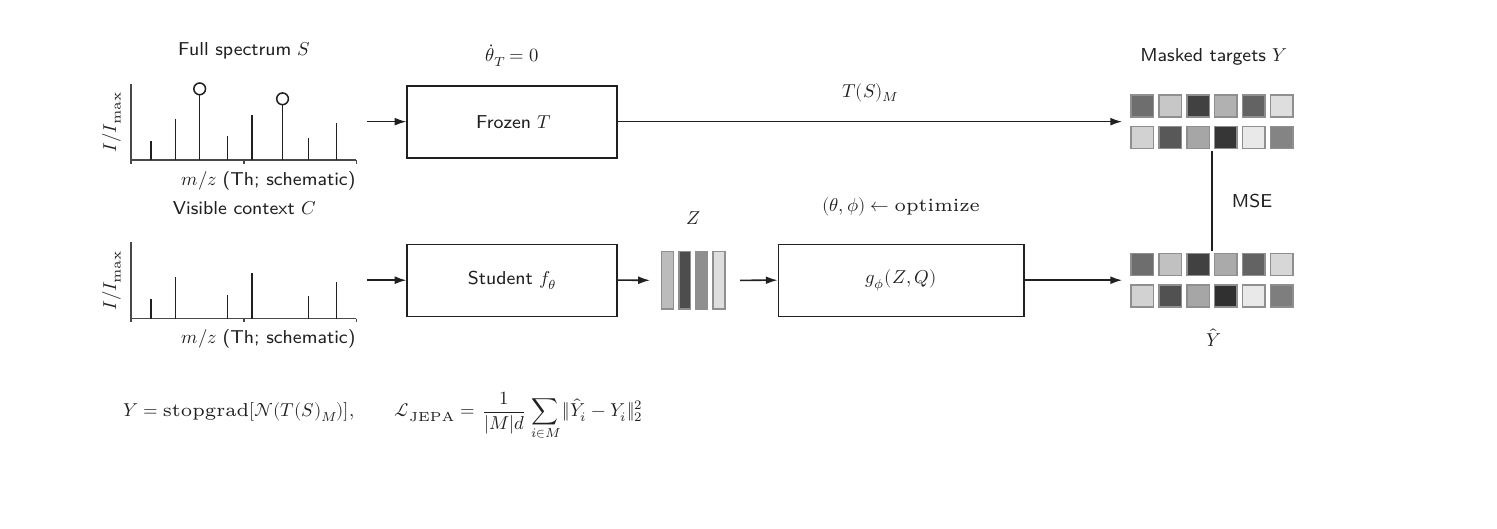
\begin{tikzpicture}[x=1cm,y=1cm,scale=1.14375,transform shape]
\node[anchor=base,inner sep=0,small] at (2.40,6.54) {Full spectrum $S$};
\begin{scope}[shift={(1.15,5.38)}]
\draw[muted,line width=.55pt] (0,0)--(2.5,0);
\draw[muted,line width=.55pt] (0,0)--(0,.85);
\draw[ink,line width=.55pt] (0.22,0)--(0.22,0.2125);
\draw[ink,line width=.55pt] (0.49,0)--(0.49,0.4590);
\draw[ink,line width=.55pt] (0.76,0)--(0.76,0.7905);
\draw[ink,line width=.55pt] (1.07,0)--(1.07,0.2635);
\draw[ink,line width=.55pt] (1.34,0)--(1.34,0.5015);
\draw[ink,line width=.55pt] (1.68,0)--(1.68,0.6800);
\draw[ink,line width=.55pt] (1.97,0)--(1.97,0.2465);
\draw[ink,line width=.55pt] (2.28,0)--(2.28,0.4080);
\draw[draw=ink,fill=paper,line width=.55pt] (0.76,0.7905) circle (.065);
\draw[draw=ink,fill=paper,line width=.55pt] (1.68,0.6800) circle (.065);
\foreach \x in {0,1.25,2.5}{\draw[muted,line width=.55pt] (\x,0)--+(0,-.04);}
\node[anchor=base east,inner sep=0,tinytext] at (2.5,-.28) {$m/z$ (Th; schematic)};
\node[rotate=90,inner sep=0,tinytext] at (-.22,.425) {$I/I_{\max}$};
\end{scope}
\coordinate (fullout) at (3.77,5.805);
\node[box,text width=2.05cm,inner xsep=4pt,minimum height=.80cm] (teacher) at (5.38,5.805) {Frozen $T$};
\draw[arr] (fullout)--(teacher.west);
\node[anchor=base,inner sep=0,font=\figurefont] at (5.38,6.47) {$\dot\theta_T=0$};
\node[anchor=base,inner sep=0,small] at (13.15,6.47) {Masked targets $Y$};
\draw[draw=ink!50,fill=ink!20,line width=.55pt] (12.250,5.510) rectangle +(.25,.24);
\draw[draw=ink!50,fill=ink!75,line width=.55pt] (12.560,5.510) rectangle +(.25,.24);
\draw[draw=ink!50,fill=ink!40,line width=.55pt] (12.870,5.510) rectangle +(.25,.24);
\draw[draw=ink!50,fill=ink!90,line width=.55pt] (13.180,5.510) rectangle +(.25,.24);
\draw[draw=ink!50,fill=ink!10,line width=.55pt] (13.490,5.510) rectangle +(.25,.24);
\draw[draw=ink!50,fill=ink!55,line width=.55pt] (13.800,5.510) rectangle +(.25,.24);
\draw[draw=ink!50,fill=ink!65,line width=.55pt] (12.250,5.860) rectangle +(.25,.24);
\draw[draw=ink!50,fill=ink!25,line width=.55pt] (12.560,5.860) rectangle +(.25,.24);
\draw[draw=ink!50,fill=ink!85,line width=.55pt] (12.870,5.860) rectangle +(.25,.24);
\draw[draw=ink!50,fill=ink!35,line width=.55pt] (13.180,5.860) rectangle +(.25,.24);
\draw[draw=ink!50,fill=ink!70,line width=.55pt] (13.490,5.860) rectangle +(.25,.24);
\draw[draw=ink!50,fill=ink!15,line width=.55pt] (13.800,5.860) rectangle +(.25,.24);
\coordinate (targetwest) at (12.15,5.805);
\coordinate (targetnorth) at (13.15,6.13);
\coordinate (targetsouth) at (13.15,5.4799999999999995);
\draw[arr] (teacher.east)--node[above=4pt,small]{$T(S)_M$}(targetwest);
\node[anchor=base,inner sep=0,small] at (2.40,4.77) {Visible context $C$};
\begin{scope}[shift={(1.15,3.62)}]
\draw[muted,line width=.55pt] (0,0)--(2.5,0);
\draw[muted,line width=.55pt] (0,0)--(0,.85);
\draw[ink,line width=.55pt] (0.22,0)--(0.22,0.2125);
\draw[ink,line width=.55pt] (0.49,0)--(0.49,0.4590);
\draw[ink,line width=.55pt] (1.07,0)--(1.07,0.2635);
\draw[ink,line width=.55pt] (1.34,0)--(1.34,0.5015);
\draw[ink,line width=.55pt] (1.97,0)--(1.97,0.2465);
\draw[ink,line width=.55pt] (2.28,0)--(2.28,0.4080);
\foreach \x in {0,1.25,2.5}{\draw[muted,line width=.55pt] (\x,0)--+(0,-.04);}
\node[anchor=base east,inner sep=0,tinytext] at (2.5,-.28) {$m/z$ (Th; schematic)};
\node[rotate=90,inner sep=0,tinytext] at (-.22,.425) {$I/I_{\max}$};
\end{scope}
\coordinate (contextout) at (3.77,4.045);
\node[box,text width=2.05cm,inner xsep=4pt,minimum height=.80cm] (student) at (5.38,4.045) {Student $f_\theta$};
\draw[arr] (contextout)--(student.west);
% Context features are vectors, not a second learned operation.
\foreach \i/\shade in {0/30,1/80,2/50,3/15}{\draw[draw=ink!50,fill=ink!\shade,line width=.55pt] (7.04+\i*.19,3.725) rectangle +(.13,.64);}
\node[anchor=base,inner sep=0,small] at (7.39,4.66) {$Z$};
\node[anchor=base,inner sep=0,font=\figurefont] at (9.7,4.81) {$(\theta,\phi)\leftarrow\mathrm{optimize}$};
\draw[arr] (student.east)--(6.91,4.045);
\node[box,text width=2.45cm,inner xsep=4pt,minimum height=.80cm] (predictor) at (9.7,4.045) {$g_\phi(Z,Q)$};
\draw[arr] (7.91,4.045)--(predictor.west);
\draw[draw=ink!50,fill=ink!20,line width=.55pt] (12.250,3.750) rectangle +(.25,.24);
\draw[draw=ink!50,fill=ink!78,line width=.55pt] (12.560,3.750) rectangle +(.25,.24);
\draw[draw=ink!50,fill=ink!40,line width=.55pt] (12.870,3.750) rectangle +(.25,.24);
\draw[draw=ink!50,fill=ink!93,line width=.55pt] (13.180,3.750) rectangle +(.25,.24);
\draw[draw=ink!50,fill=ink!10,line width=.55pt] (13.490,3.750) rectangle +(.25,.24);
\draw[draw=ink!50,fill=ink!58,line width=.55pt] (13.800,3.750) rectangle +(.25,.24);
\draw[draw=ink!50,fill=ink!65,line width=.55pt] (12.250,4.100) rectangle +(.25,.24);
\draw[draw=ink!50,fill=ink!28,line width=.55pt] (12.560,4.100) rectangle +(.25,.24);
\draw[draw=ink!50,fill=ink!85,line width=.55pt] (12.870,4.100) rectangle +(.25,.24);
\draw[draw=ink!50,fill=ink!38,line width=.55pt] (13.180,4.100) rectangle +(.25,.24);
\draw[draw=ink!50,fill=ink!70,line width=.55pt] (13.490,4.100) rectangle +(.25,.24);
\draw[draw=ink!50,fill=ink!18,line width=.55pt] (13.800,4.100) rectangle +(.25,.24);
\coordinate (predictionwest) at (12.15,4.045);
\coordinate (predictionnorth) at (13.15,4.37);
\coordinate (predictionsouth) at (13.15,3.72);
\draw[arr] (predictor.east)--(predictionwest);
\node[anchor=base,inner sep=0,small] at (13.15,3.31) {$\widehat Y$};
\draw[ink,line width=.55pt] (predictionnorth)--node[right=4pt,small]{MSE}(targetsouth);
\node[anchor=base west,inner sep=0,font=\figurefont] at (1.05,2.53) {$\displaystyle Y=\sg[\mathcal N(T(S)_M)],\qquad\mathcal L_{\rm JEPA}=\frac{1}{|M|d}\sum_{i\in M}\|\widehat Y_i-Y_i\|_2^2$};
% Fixed canvas: 183 x 60.046875 mm. No clipping: overflow is audited.
\pgfresetboundingbox
\path[use as bounding box] (0,1.6) rectangle (16,6.85);
\end{tikzpicture}
\end{document}
